\chapter{Modular Anomaly Detection Framework}
\label{chapter:Chapter 3}
\lhead{Chapter 3. \emph{Methods and Systems Developed}}

In this Chapter, we present the proposed Modular Anomaly Detection Framework. Firstly list the actual requirements that served as a blueprint for the developed Framework. This requirements were either defined by Maritime Officer Experts under the MARISA project, or from limitations from the Data either from the  

Second we show the proposed Modular Anomaly Detection Framework, as shown in Fig. XX. And in the following sections we provide a overall explanation of each module functionality. 

by describing the overall view of the proposed Modular Framework, Secondly we provide a detailed explanation of each Module and the methods used for each Module. 

\section{Framework Requirements}
\label{section: Framework Requirements}
In order to develop a framework that will addresses the real demands of Maritime Officers, we surveyed the only agents that could significantly insight Maritime Officers under the MARISA project. in order to fully understand the demands for a Framework for Maritime Anomaly Detection.
This being said, for the defined requirements we categorized them into three main classes:

\begin{description}
\item[Anomalies Requirements] Having the concept of Behavioural Vessel Anomaly defined by Maritime Officers is the most reliable way to define an anomaly at Seas. Therefore, Maritime Officers defined a list of Anomalies, in which we developed methods to detect those anomalies. 

Being the one truly viable method to define of the methods we used to detect anomalies in the data, 
sequence of features is transformed into a feature vector, then convectional classification methods are applied. Feature selection represents is an important task for this method of classification.

\item [Functional Requirements] As the developed Framework was implemented so it could be used by Maritime Authorities, it was completely mandatory that the Framework could be not only deployed in different environment, but also completely modular and scallable; as different Maritime Authorities have different requirements. 
not controlled by us.

\item [Data Requirements] This requirements, were the class of requirements were not so obvious to classify. Any Framework that deals with Maritime data, is certain that it needs to be implemented so it can handle really high workflows of data, due to the increasing volume of Vessels at Seas. Although, Maritime is represented by different types of data from Meteo data to AIS data to even Fishing logs data, which come in different structures, or even with no structure at all.
\end{description}

\todo[inline]{NEED A TABLE OR SOMETHING WITH THE ACTUAL REQUIREMENTS}


\section{Proposed Framework}
In order to develop a Framework capable of addressing the requirements defined, above in \ref{section: Framework Requirements}, we propose a Modular Vessel Anomaly Detection Framework, able to ingest data from different feeds in real-time data, construct a Data-Base for Vessels Trajectories in a unsupervised manner, and detect different Anomalies over either real-time incoming data or stored Vessels Trajectories; as it is represented in \ref{fig:Framework}.

We provide a Modular Framework, as there are no inputs or outputs absolute standards nor defined requirements for any Framework for Anomaly Detection on the Maritime domain, so by providing a configurable and specially not static Framework, we provide the flexibility for providing the same Framework configured for different scenarios or even different National Maritime Authorities.

as the requirements for one so by defining a Framework allows a flexible configuration from either types of Anomalies, system, allows a easier adoption of these services by Maritime end users. 

on a Lambda Architecture, and having the Apache Ecosystem. composed from four main modules, as shown in Fig. XX ...

\begin{figure}[H]
	\centering
	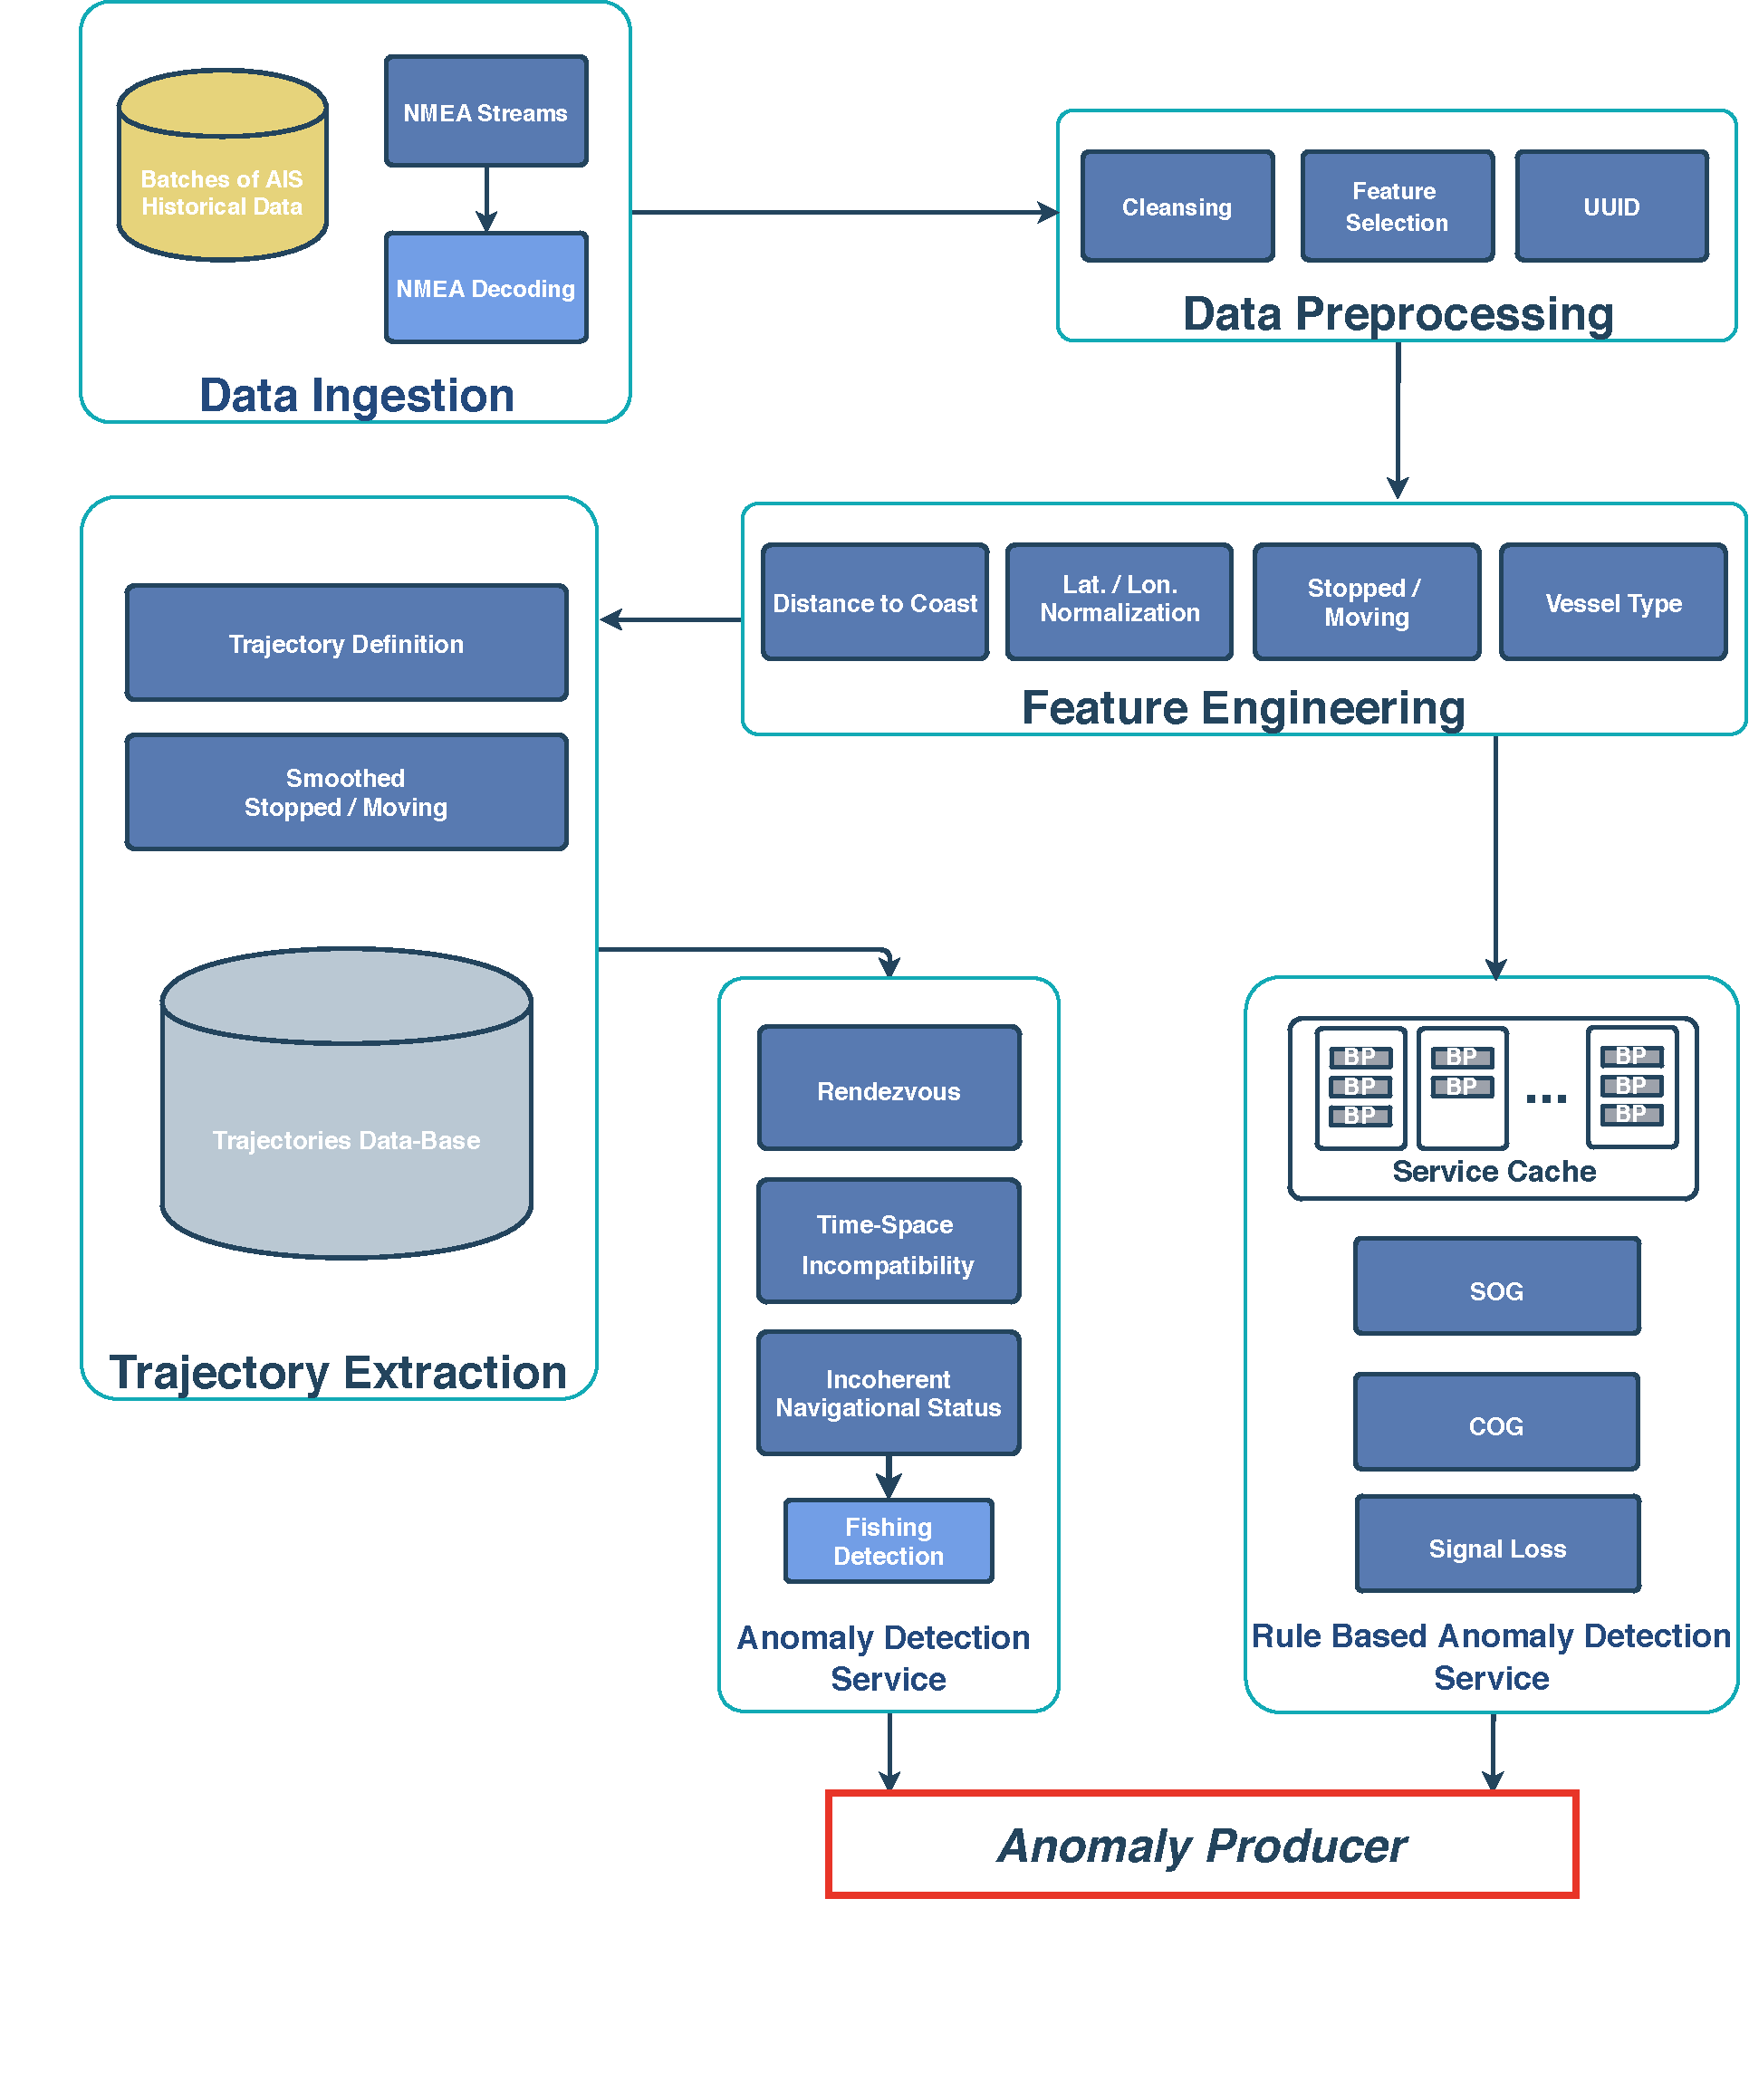
\includegraphics[scale = .37]{figures/Ch3/Framework.pdf}
    \caption{Proposed Beta Framework \todo[inline]{NEEDS MORE DETAIL THIS IMAGE}.}
    \label{fig:Framework}
\end{figure}

In the following subsections, we discuss each module: Data Fusion, Vessel T Extraction, Anomaly Detection and Reporting...

\section{Data Ingestion}
Data Ingestion Module, represents the Data input for the developed Framework. AIS data was the most representative data type used for this work, as it showcases the actual instantaneous Vessel information.
Although, used AIS data for this work came in two really distinct formats: It came either in \textbf{Historical Batches} representing Historical sets of Data, or real \textbf{NMEA AIS Streams}, representing real, real-time 
data.

AIS Historical Data-Sets, can be found in open-access repositories, although Historical AIS Data providers cap the frequency of the messages transitions. This drastically reduces the number of transmitted messages, but also reduces the overall detail of the Data, as lower transmissions rates produce a less certainty of the movement presented by each Vessel. Which, for most general uses of AIS (e.g. managing a fleet, estimations of time of arrival ...), transmissions rates of 3 Seconds vs 30 Seconds, do not provide any information gain, as Vessel kinematics tend to not change abruptly in short periods of time. 

Although, via the MARISA project, we received AIS data via live feeds from Antennas all around the European coast. This Antennas receive the Vessels transmissions broadcast via AIS, till normally a range of 20 Nautical Miles of the shore and depending on the live feed provider, AIS messages can be received in rates up to 30 Messages per Minute per Vessel. This type of incoming Data Streams represents the Real scenario, in which the Framework will be tested. Real live streams of AIS data, are received via TCP stream in NMEA format which in order to be represented as AIS messages required to be decoded, which is described in the subsection under.


\subsection{NMEA Data Streams}
National Marine Electronics Association (NMEA) is a standard communication protocol used by Maritime Sensors such as Accelerometer, Giroscope, GPS receivers, etc.
NMEA encapsulates the information from the different Vessel sensors, and broadcasts this information

being the standard it is the protocol that encapsulates the AIS information, broadcasted by AIS-equipped Vessels. 

\begin{figure}[H]
	\centering
	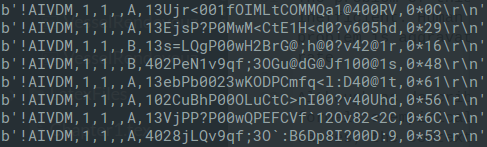
\includegraphics[scale = .5]{figures/Ch3/NMEAexample.png}
    \caption{Snapshot of raw AIS data in NMEA format.}
    \label{fig:NMEAexample}
\end{figure}

\todo[inline]{TODO SAME AS IN TOP ITS BS}

Via the project, we had access to multiple live NMEA feeds, as a way to not only validate our developed methods with live feeds of Nautical data, but also to produce methods that were capable of handling the scale of data that is produced by National feeds.

The use of real data comes with many challenges, as it is mandatory to decode sort and store this data in order to de accessed as a viable source of data; a snapshot of a example of a NMEA feed can be found in Figure \ref{fig:NMEAexample}. 

\todo[inline]{this might go to chap4}

AIS-Receiving stations receive the broadcast AIS information from numerous AIS-equipped Vessels simultaneously. Normally, AIS-Receiving stations are antennas located along the coast line in high grounds, the reception range of these antennas vary, mainly depending on distance to shore, the elevation in which the antenna is located, and the antenna type itself.

Although, the distance in which Stations are capable of receiving AIS messages presents a problem to the Data, as reception ranges vary from 15 Nautical Miles to 50 Nautical Miles, this creates the problem of 

\begin{enumerate}
\item Duplication of Reception:  With the variation of reception ranges, it frequently occurs that multiple stations, receive the same  

\todo[inline]{THIS BRINGS TO THE PROBLEM OF MULTIPLE ANTHENAS RECEIVING THE SAME FEED... disse que havia dois problemas}

\end{enumerate}

\subsection{Data Storage}
With NMEA streams producing enormous workflows of data, the storage of becomes a problem for the developed Framework, as it must not only decode and process the NMEA feeds but also store the decoded messages, in a "very fast" and scalable way.

Thus, and as requirement of the MARISA project was to use Apache Spark [REF FOR APACHE SPARK] modules for data-ingestion and pre-processing, we decided to use Apache Cassandra as the Data-Storage for the proposed framework.

technology has provides a lightweight solution for storage of enormous flows of Data, but also 
enoumoit stacks well with Apache Spark...


the report anomalies, it made the choose of A

of choosing a technology that can Store this information in a not only 'very fast' way but also storage of this Data after is processed 

\section{Data Pre-processing}
Data Pre
\section{Feature Engineering}
Feature Engineering presents a crucial step for any machine learning project, as selecting the right features that better represent the data, directly influences any result generated by the model.  
As described in Section \ref{subsection: chp2_AIS}, AIS presents a large amount of different features. This creates a problem of estimating the use-fullness of each feature provided in by the AIS, as it requires a pre-conceived knowledge of the used data, that is only acquired with the experience in the Maritime domain.

Thus for this Framework, the choice of most suitable features that represent a Vessels movement was based on the literature and with the help of Maritime Knowledge Expert. Which lead to the choice of the features that solely represent the Vessels kinematics.

We further enrich our features in two ways, firlty by analyzing each AIS message as point aas a single point in Time and calculating aditional distances, such as distance to shore and distance to the most near Port.

each point in t the represented features of each message by by doing a point based analysis, in which we concidered the information of  

by normalizing the Latitude and Longitude features of each position, calculating the Distance to Shore and the kinematic features that represent the instantaneous move-state of the Vessel. Every calculation is done a priory, thus enhancing the performance and reliability of the Anomaly Detection Modules, which are explained in detail in section \todo{REF TO SECTION!}

% \section{Unsupervised Vessel Route Extraction}
\section{Vessel Trajectory Definition}
In this Section we present our definition our interpretation and formulation of Vessel Trajectory, 
Representing a Vessel Trajectory data, can become a difficulty in the Maritime domain. Currently there are a vast number of solutions described in the literature, presenting different solutions for different types of problems. 

Our approach to represent a Maritime trajectory, was to consider a trajectory as a whole, this is, as Vessel are obliged to broadcast their AIS information in a semi-continuous rates; knowing that each AIS broadcast message represent the instantaneous kinematic information from a Single Vessel, aggregating this information over time will represent a Vessel Trajectory. 

Thus, by identifying each vessel by its unique identifier (MMSI), the trajectory can be considered as the set of AIS messages, identified by the MMSI of each Vessel.

\begin{figure}[H]
	\centering
	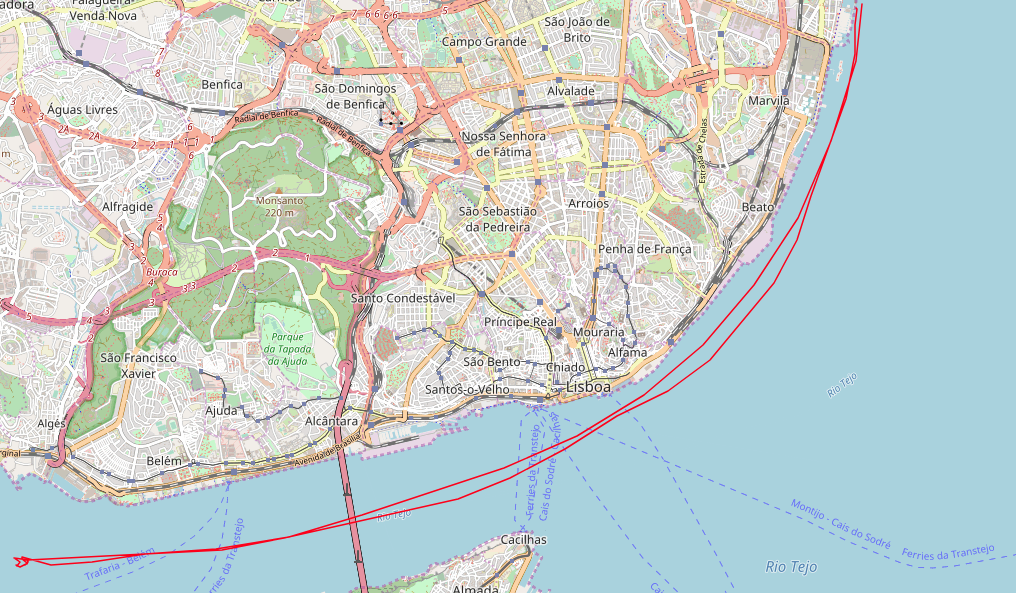
\includegraphics[scale = .3]{figures/Ch3/traj_example.png}
    \caption{Trajectory snapshot(2017-11-05 10:22 to 2017-11-05 22:42) from Vessel MMSI: 255806006}
    \label{fig: TrajectorySMM_example}
\end{figure}

Although, as each AIS message is time-stamped(contains the time in which was broadcast), our representation of trajectory can be defined as Multivariate Time-Series, this is for each trajectory we have $N$ time-series, in which $N$ represents the number of features considered for each trajectory, further explained in the subsections bellow.

\subsection{Feature Engineering}
Feature Engineering presents a crucial step for any machine learning project, as selecting the right features that better represent the data, directly influences any result generated by the model.  
As described in TODO chapter X TODO,  AIS presents a large amount of different features. This creates a problem of estimating the use-fullness of each feature provided in by the AIS, as it requires a pre-conceived knowledge of the used data. 

Thus, for this work the choice of most suitable features that represent a Vessels movement was done with the help of Maritime Knowledge Expert. Which lead to the choice of the features that solely represent the Vessels kinematics.

which directly increases or decreases the complexity of the  is not a trivial task, it requires a pre-conceived knowledge of the used data, and more important expectation of the    as not every feature has the same relevancy, thus 

ant for the 

the problem by having an enormous amount of features,  is that the estimation of the usefulness of the features 

it most of these features donot represent any which might bring 

a presents different possibilities analysis, as it contains detailed information the actual Vessel Behaviour. Although for this work we focused, on the information that more characterize the Vessel kinematics behaviour, thus decreasing the number of features we have in our Data-Model.

\subsection{Multivariate Time-Series Analogy}
As mentioned above, each Trajectory is considered as a Time Series composed of Multiple features.  

in Fig. \ref{fig: MTimeSeries_example}, we represent the Vessel trajectory showend in figure X. 
For each trajectory we consider the features representing 
main features that a which in order to normalize our analysis of a Vessel Route, we ...
\todo[inline]{TODO dar palha para introduzir esta imagem}

\begin{figure}[H]
	\centering
	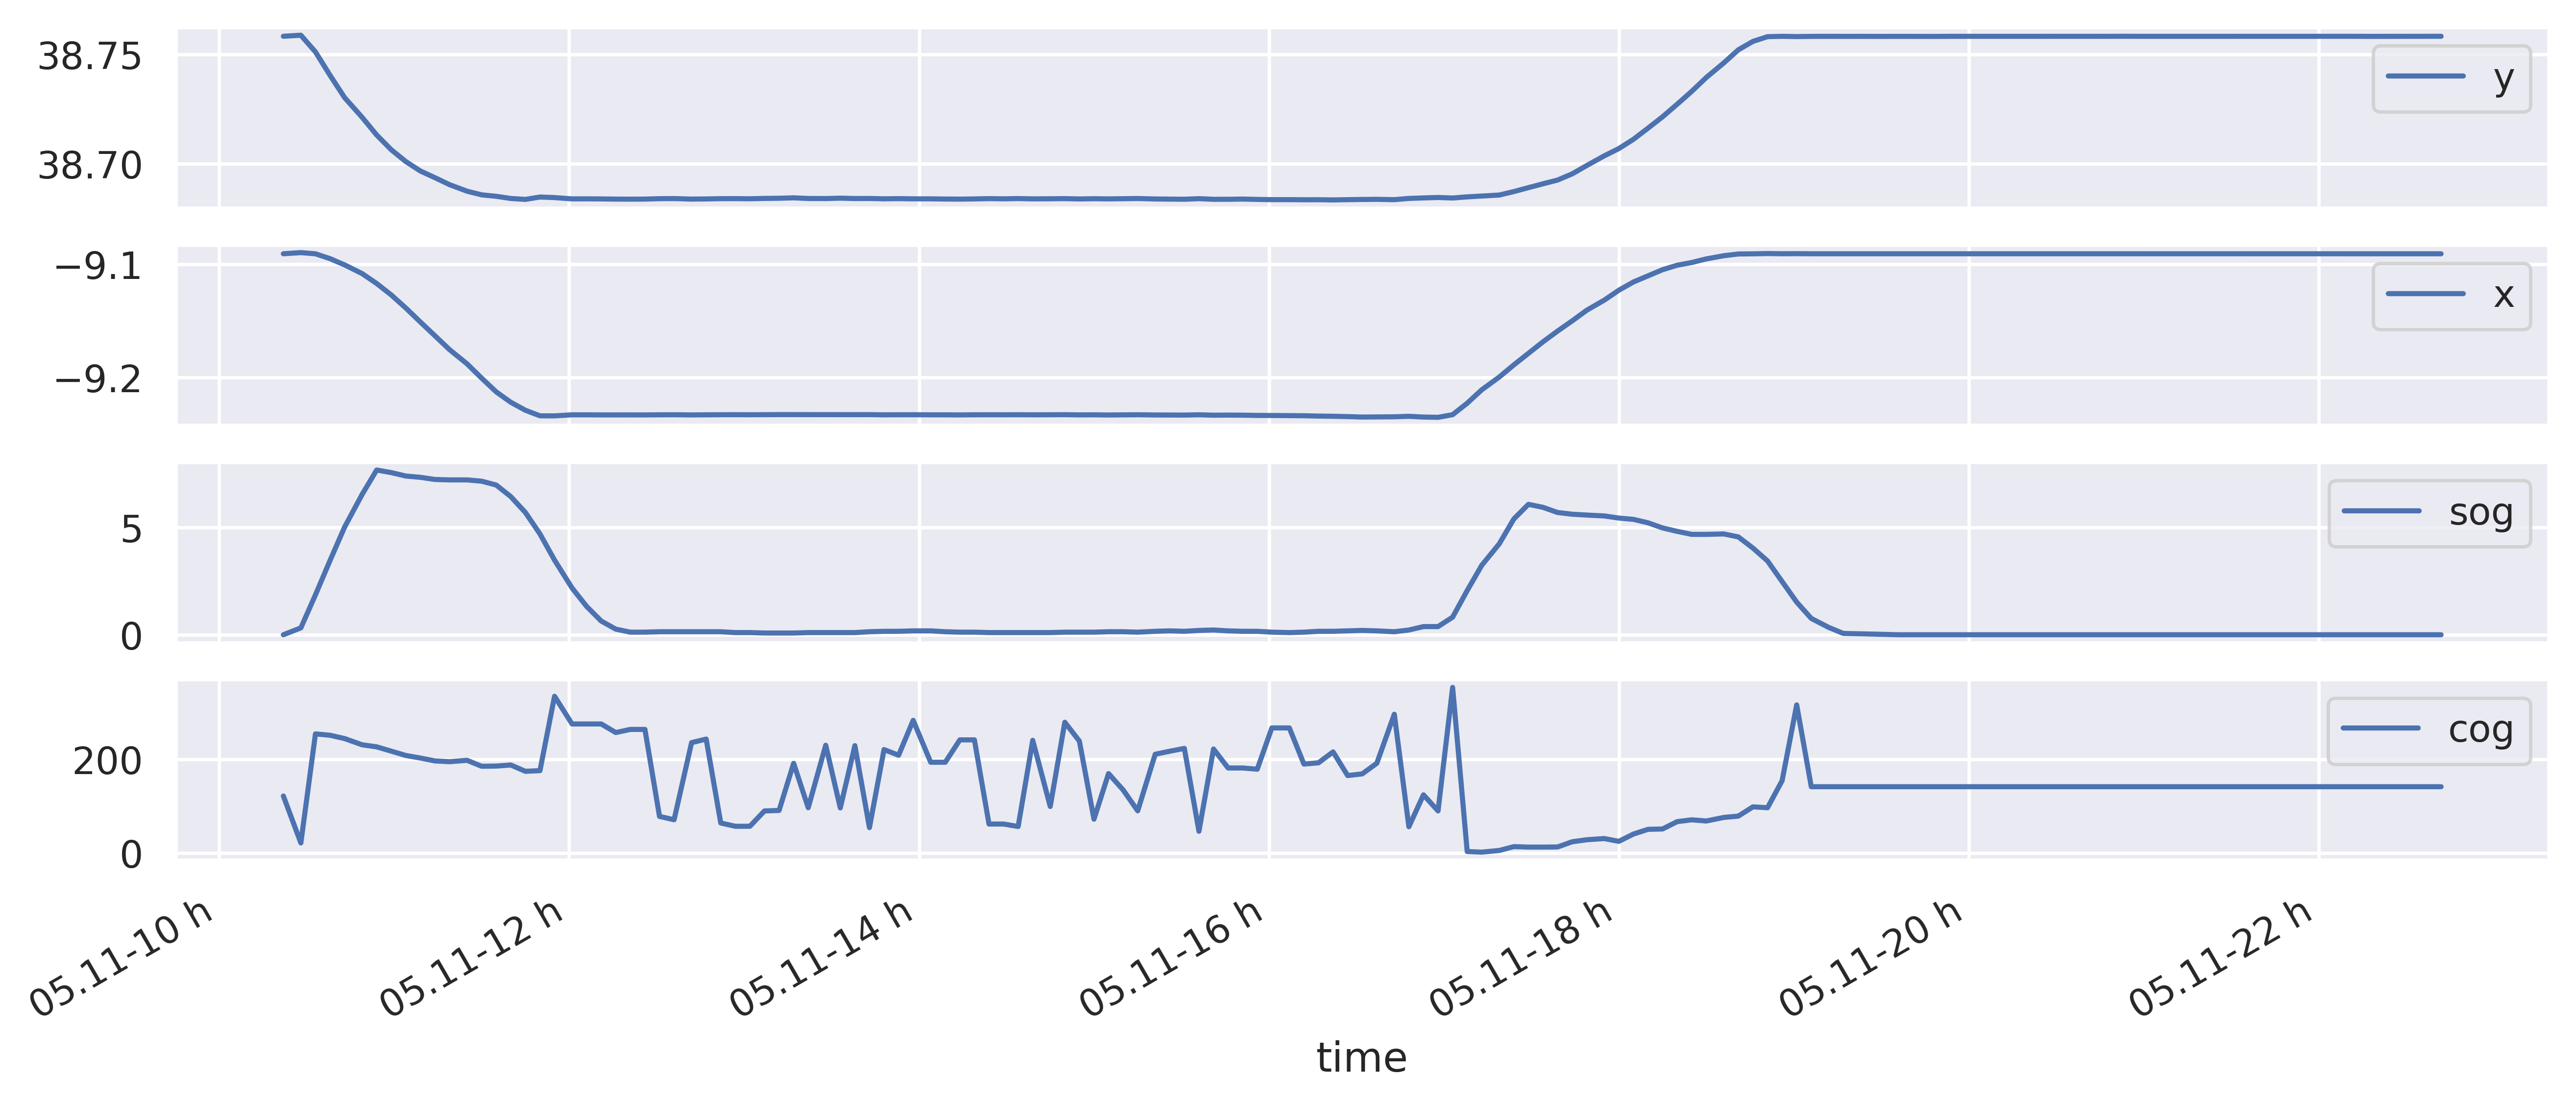
\includegraphics[scale = .5]{figures/Ch3/ts_example.png}
    \caption{Trajectory represented in Fig.X, presented as a Multivariate Time Series.}
    \label{fig: MTimeSeries_example}
\end{figure}


\section{Anomaly Definition}
An Anomaly can have numerous interpretations depending on the context in which is found, but it can be generally defined as Data that stand out when contrasted to other Data.

Nowadays Vessel Anomaly Detection is solely done by Human Maritime Experts, with every Maritime Security Agency assuring the coastal surveillance of their territory, by assessing possible threats, and identifying abnormal behaviour. 
%The identified abnormal Vessel behaviour is then further investigated by Maritime Authorities, which can lead to fines or even criminal charges against the Vessel crew. 
The problem of this current methodology for Anomaly Detection, is that is extremely inefficient. Human analysis only allows a limited number of Vessels that can be analyzed. This problem is aggravated as the number of Vessel at seas is increasing every year in a exponential rate. 

This creates a typical situation for the use of Machine Learning models to aid the necessities of Maritime Experts.
%, in the field of Maritime Anomaly Detection.
Although, formalizing an Vessel Anomalous Behavior is extremely difficult, as it is not clear what is Anomalous in the when only analyzing the Maritime data, and there is no available historical Anomalous Data-Set, to the best of our knowledge.

To solve this problem of the defining Vessel Abnormal Behaviour, Expert Knowledge from Maritime Experts was accessed under the MARISA project. Maritime Experts in order to define Anomalies which could be formalized, provided a list of Vessels Anomalies which behaviour. firstly a list of  



%It is impossible to define Anomalous, when only   

%any Vessel Anomaly can be caused by a undetermined number of factors,      . 

Thus, the context and causes of every Anomaly needs defined by Maritime Experts. Thus, in order to surpass the problem of the definition of an Anomaly; Expert Knowledge from Maritime Experts was accessed under the MARISA project. Maritime Experts defined, firstly a list of  




